\documentclass[a4paper,norsk]{article}
\usepackage{preamble}

\begin{document}
\maketitle

\section*{Introduction of problem}
Consider an infinite rotating disk placed at z=0 under a newtonian viscous fluid initially at rest,
viscous forces will set up a rotating velocity field in the fluid. von Karman(1) showed that the steady state flow
of this problem could be reduced to a set of ordinary differential equations. He solved them by
approximate integration method, which will be used as reference for the CFD results in this test.

\begin{figure}[h!]
	\centering
	\caption*{Spinning circle}
	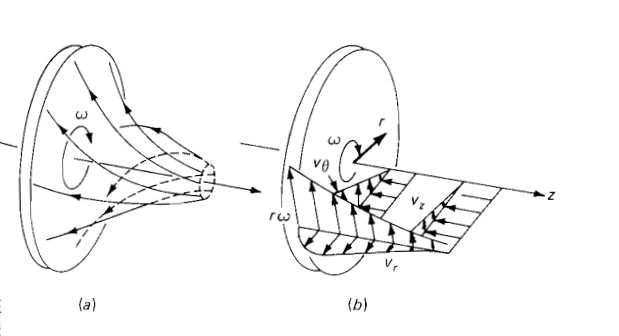
\includegraphics[scale=0.6]{VonKarman.png}
\end{figure}

\section*{Theory}
Let the velocity vector components be defined as $\textbf{v} = (v_r, v_\theta, v_z)$
By the assumption of radial symmetry, we expect our components to be independent of the angle \textbf{$\theta$}.
The continuity equation for a polar coordinate system in accordance with our assumption is defined by
\begin{align}
\nabla \cdot \textbf{v} = \frac{1}{r} \frac{\partial(r v_r)}{\partial r} +
                        \frac{\partial v_z}{\partial z} = 0
\end{align}

Moving on to the equation of momentum, the familiar Navier-Stokes equation yields.
\begin{align}
\frac{\partial \textbf{v}}{\partial t} + \textbf{v} \cdot \nabla \textbf{v} &=
-\frac{\nabla p}{\rho} + \frac{\mu}{\rho} \nabla^2 \textbf{v}
\end{align}

Considering steady-flow we end up with the following component equations.
\begin{align}
r &: \hspace{1cm} v_r\frac{\partial v_r}{\partial r} - \frac{v_\theta^2}{r} + v_z\frac{\partial v_r}{\partial z}
= -\frac{1}{\rho} \frac{\partial p}{\partial r} + \frac{\mu}{\rho}( \frac{\partial^2 v_r}{\partial r^2} +
\frac{1}{r} \frac{\partial v_r}{\partial r} + \frac{\partial^2 v_r}{\partial z^2} - \frac{v_r}{r^2} ) \\
\theta &: \hspace{1cm} v_r\frac{\partial v_\theta}{\partial r} + v_z\frac{\partial v_\theta}{\partial z} +
\frac{1}{r}v_\theta v_r = \frac{\mu}{\rho} (\frac{\partial^2 v_\theta}{\partial r^2} +
\frac{1}{r} \frac{\partial v_\theta}{\partial r} + \frac{\partial^2 v_\theta}{\partial z^2} -
\frac{v_\theta}{r^2} ) \\
z &: \hspace{1cm} v_r \frac{\partial v_z}{\partial r} + \frac{\partial v_z}{\partial z} =
\frac{1}{\rho} \frac{\partial p}{\partial z} + \frac{\mu}{\rho} (\frac{\partial^2 v_z}{\partial r^2} +
\frac{1}{r} \frac{\partial v_z}{\partial r} + \frac{\partial^2 v_z}{\partial z^2}
)
\end{align}

For our problem we define the following boundary conditions.

\begin{itemize}
\item On disk surface $$v_r = 0, v_\theta = r\Omega, v_z = 0$$
\item Disk circumference $$\frac{\partial}{\partial r} (\frac{v_r}{r}) = 0,
\frac{\partial}{\partial r} (\frac{v_\theta}{r}) = 0,
 \frac{\partial v_z}{\partial r} = 0$$
\item End of integration domain $$v_r = 0, v_\theta = 0, \frac{\partial v_z}{\partial z} = 0 $$
\end{itemize}

Introducing von Karman's substitutions of the velocity components,

\begin{align*}
v_r = r \omega F(\zeta) \hspace{2mm} v_\theta = r \omega G(\zeta) \hspace{2mm}
v_z = (\nu \omega )^{\frac{1}{2}} H(\zeta) \\
p = \rho \nu \omega, \hspace{4mm} \zeta = (\omega/ \nu)^{\frac{1}{2}} z
\end{align*}

we can rewrite (3-5) as a system of ODE's as follows

\begin{align}
F^2 - G^2 + HF^{'} &= F^{''} \\
2FG + HG^{'} &= G^{''} \\
2F + H^{'} &= 0 \\
P^{'} +2F^{'} &= -HH^{'} \\
\end{align}

The corresponding boundary conditions yields

\begin{itemize}
\item $F = 0, \hspace{3mm} G = 1, \hspace{3mm} H = -a$ \hspace{3mm} at $\zeta = 0 $
\item $F = 0, \hspace{3mm} G = 0 \hspace{3mm}$ at $\zeta = \infty $
\end{itemize}

\section*{Solving the problem}
For the presented problem, the Navier-Stokes solver Oasis based on the FEniCS software will be used
to solve the PDE system using finite element method. \newline
For the computation we have to construct a mesh to do our calculations upon. In this problem we will use
Gmsh, a free 3D finite element grid generator. The problem will be solved on a pipe with r = 1 and height
z = 3. The pipe will be constructed with denser elements at the spinning boundary, as seen in the presented
figure.

\begin{figure}[h!]
	\centering
	\caption*{Pipe mesh}
	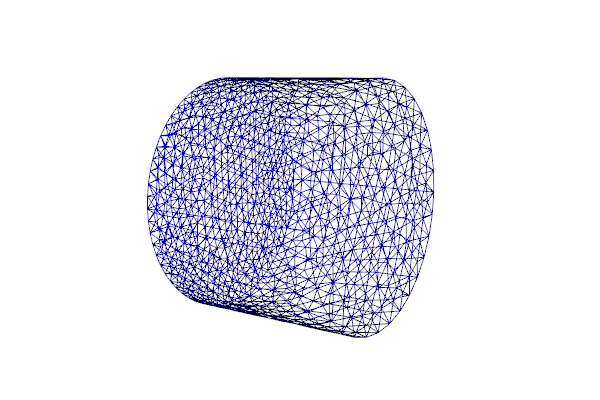
\includegraphics[scale=0.6]{pipe.png}
\end{figure}

\newpage

Continuing on the reference solution, we derive Karman's method of approximate solution.
Firstly we want to observe how the differential equations behave at the limit $\zeta \rightarrow \infty$.
Assuming H approaches a limit $-c$ as while $F, G \rightarrow $ as $\zeta \rightarrow \infty$, we end
up with the following relations for large $\zeta$.
\begin{align}
-cG^{'} &= G^{''} \hspace{3mm} -cF^{'} = F{''} \\
F &= Ae^{-c\zeta}, \hspace{3mm} G = Be^{-c \zeta}, \hspace{3mm} H = -c + \frac{2A}{c}e^{-c\zeta}
\end{align}
As we can see, F and G approaches 0 exponentially, and we can assume they are 0 for some value of $\zeta$
which we will call $\zeta_0$.
This will be exploited in the following integration scheme.

Starting by integrating equation (6)-(7)from 0 to $\infty$, and using relation (8).

\begin{align*}
\int_0^\infty HF^{'} d\zeta = \big[HF \big]_0^\infty - \int_0^\infty H^{'}F d\zeta
&= 2\int_0^\infty F^2 d\zeta \\
\int_0^\infty HG^{'} d\zeta = \big[HG \big]_0^\infty - \int_0^\infty H^{'}G d\zeta
&= 2\int_0^\infty FG d\zeta
\end{align*}

Combining these results with (12), we end up with the following result

\begin{align}
-F^{'}(0) &= \int_0^\infty (3F^2 - G^2) d\zeta \\
-G^{'}(0) &= 4 \int_0^\infty FG d\zeta
\end{align}

As Karman, we assume that due to the expoential growth that F and G are zero for
values of $\zeta$ greater than $\zeta_0$. As a result
\begin{align}
F(\zeta_0) = 0, \hspace{3mm} F^{'}(\zeta_0) = 0, \hspace{3mm}
G(\zeta_0) = 0, \hspace{3mm} G'(\zeta_0) = 0
\end{align}

We can now also find $F{''}(0)$ and $G^{''}(0)$ by setting $\zeta = 0$ in the system of ODE's

\begin{align}
F^{''}(0) = -1 \hspace{3mm} G^{''}(0) = 0
\end{align}

Now if we let $F^{'}(0)$ is some constant \textit{a}, the following functions fulfills equation (15)-(16) and
the boundary conditions.

\begin{align}
F &= (1 - \frac{\zeta}{\zeta_0})^2 \hspace{2mm} \big(a\zeta + (\frac{2a}{\zeta_0}) \zeta^2 \big) \\
G &= (1 - \frac{\zeta}{\zeta_0} )^2 \hspace{2mm} (1 + \frac{\zeta}{2\zeta_0} )
\end{align}

This yields $G^{'}(0) = -\frac{3}{2 \zeta_0}$. Inserting (17)-(18) in (13)-(14), we get a system of
equations to solve a and $\zeta_0$.

\newpage
\section*{Computations}
\begin{center}
    \begin{tabular}{| l | l | l | l | l | l | p{5cm} |}
    \hline
    $\zeta$ & F & F' & G & G' & H & -P \\ \hline
    0.0 & 0.0 & 0.51023 & 1.00 & -0.61592 & 0.0 & 0.0 \\ \hline
	0.1 & 0.0462 & 0.4163 & 0.9386 & -0.6112 & -0.0048 & 0.0924 \\ \hline
	0.2 & 0.0836 & 0.3338 & 0.8780 & -0.5987 & -0.0179 & 0.1674 \\ \hline
	0.3 & 0.1133 & 0.2620 & 0.8190 & -0.5803 & -0.0377 & 0.2274 \\ \hline
	0.4 & 0.1364& 0.1999 & 0.7621 & -0.5577 & -0.0628 & 0.2747 \\ \hline
	0.5 & 0.1536& 0.1467 & 0.7075 & -0.5321 & -0.0919 & 0.3115 \\ \hline
	0.6 & 0.1660& 0.1015 & 0.6557 & -0.5047 & -0.1239 & 0.3396 \\ \hline
	0.7 & 0.1742& 0.0635 & 0.6067 & -0.4763 & -0.1580 & 0.3608 \\ \hline
	0.8 & 0.1789& 0.0317 & 0.5605 & -0.4476 & -0.1933 & 0.3764 \\ \hline
	0.9 & 0.1807& 0.0056 & 0.5171 & -0.4191 & -0.2293 & 0.3877 \\ \hline
	1.0 & 0.1801& -0.0157 & 0.4766 & -0.3911 & -0.2655 & 0.3955 \\ \hline
	\hline
    \end{tabular}
\end{center}


\section*{Comments}


\end{document}
